%iffalse
\let\negmedspace\undefined
\let\negthickspace\undefined
\documentclass[journal,12pt,onecolumn]{IEEEtran}
\usepackage{cite}
\usepackage{amsmath,amssymb,amsfonts,amsthm}
\usepackage{algorithmic}
\usepackage{graphicx}
\usepackage{textcomp}
\usepackage{xcolor}
\usepackage{txfonts}
\usepackage{listings}
\usepackage{enumitem}
\usepackage{mathtools}
\usepackage{gensymb}
\usepackage{comment}
\usepackage[breaklinks=true]{hyperref}
\usepackage{tkz-euclide} 
\usepackage{listings}
\usepackage{gvv}                                        
\def\inputGnumericTable{}                                 
\usepackage[latin1]{inputenc}                                
\usepackage{color}                                            
\usepackage{array}                                             
\usepackage{longtable}                                       
\usepackage{calc}                                             
\usepackage{multirow}                                         
\usepackage{hhline}                                           
\usepackage{ifthen}                                           
\usepackage{lscape}
\usepackage{multicol}

\newtheorem{theorem}{Theorem}[section]
\newtheorem{problem}{Problem}
\newtheorem{proposition}{Proposition}[section]
\newtheorem{lemma}{Lemma}[section]
\newtheorem{corollary}[theorem]{Corollary}
\newtheorem{example}{Example}[section]
\newtheorem{definition}[problem]{Definition}
\newcommand{\BEQA}{\begin{eqnarray}}
\newcommand{\EEQA}{\end{eqnarray}}
\newcommand{\define}{\stackrel{\triangle}{=}}
\theoremstyle{remark}
\newtheorem{rem}{Remark}
\begin{document}

\bibliographystyle{IEEEtran}
\vspace{3cm}

\title{NCERT - 6.5.14}
\author{EE224BTECH11044 - Muthyala koushik
}
\maketitle
\bigskip

\renewcommand{\thefigure}{\theenumi}
\renewcommand{\thetable}{\theenumi}
\textbf{\section{APPLICATION OF DERIVATIVES}}


\textbf{Question:} Find two positive numbers $x$ and $y$ such that $x + y = 60$ and $xy^3$ is maximized. \\

\solution

Let $z = xy^3$. From the equation $x + y = 60$, we can express $x$ as:  
\begin{align}
    x = 60 - y.
\end{align}

Substitute this into $z$:  
\begin{align}
    z &= xy^3 = (60 - y) \cdot y^3, \\
    z &= 60y^3 - y^4.
\end{align}

To maximize $z$, we take its derivative with respect to $y$ and set it equal to zero:  
\begin{align}
    \frac{dz}{dy} &= \frac{d}{dy}(60y^3 - y^4), \\
    \frac{dz}{dy} &= 180y^2 - 4y^3, \\
    \frac{dz}{dy} &= y^2(180 - 4y).
\end{align}

Setting $\frac{dz}{dy} = 0$:  
\begin{align}
    y^2(180 - 4y) = 0.
\end{align}

This gives two possibilities:  
\begin{itemize}
    \item $y^2 = 0 \implies y = 0$ (not valid as $y > 0$), and
    \item $180 - 4y = 0 \implies y = 45$.
\end{itemize}

Substituting $y = 45$ into $x + y = 60$:  
\begin{align}
    x = 60 - 45 \implies x = 15.
\end{align}

To confirm this is a maximum, calculate the second derivative of $z$:  
\begin{align}
    \frac{d^2z}{dy^2} &= \frac{d}{dy}(180y^2 - 4y^3), \\
    \frac{d^2z}{dy^2} &= 360y - 12y^2.
\end{align}

At $y = 45$:  
\begin{align}
    \frac{d^2z}{dy^2} &= 360(45) - 12(45^2), \\
    \frac{d^2z}{dy^2} &= 16200 - 24300, \\
    \frac{d^2z}{dy^2} &= -8100.
\end{align}

Since $\frac{d^2z}{dy^2} < 0$, the value of $z$ is maximized at $y = 45$. \\

\textbf{Final Answer:} The two numbers are $x = 15$ and $y = 45$.\\


\textbf{Solution by the method of Gradient Descent:}
Using the the method of gradient accent;
\begin{align}
	y_{n+1}=y_n+h*F^{'}(y_n)
\end{align}

from the equation above:
\begin{align}
	y_{n+1}=y_n+h*\brak{{y_n}^2\brak{180-4y_n}}
\end{align}
 
Choosing $y_0=20$, $\alpha=0.0001$, we get thave value of y as,\\
x value at maxima =  15.00000114024828\\
y value at maxima =  44.99999885975172\\


 \textbf{Solution using geometric programming:}\\
Geometric programming deals with problems where the objective and constraints are expressed as posynomials or monomials. 

A monomial is of the form:
\begin{align}
    {x_1}^{a_1}{x_2}^{a_2}\cdots{x_n}^{a_n},
\end{align}
where $x_1, x_2, \dots, x_n$ are variables, and $a_1, a_2, \dots, a_n$ are real constants.

A posynomial is a sum of monomials with non-negative coefficients:
\begin{align}
    f(x_1, x_2, \dots, x_n) = \sum_{i=1}^N c_i \prod_{j=1}^n x_j^{a_{ij}},
\end{align}
where $c_i \geq 0$.

The optimization problem is:
\begin{align}
    \text{Minimize: } & f(x_1, x_2, \dots, x_n), \\
    \text{Subject to: } & g_i(x_1, x_2, \dots, x_n) \leq 1, \quad i = 1, 2, \dots, m,
\end{align}
where $g_i(x_1, x_2, \dots, x_n)$ are posynomials.

For $f(x, y) = xy^3$, it is a monomial:
\begin{align}
    f(x, y) = x^1 y^3.
\end{align}

The Lagrangian for an objective function $f(x, y)$ and a constraint $g(x, y)$ is given by:
\begin{align}
    L(x, y, \lambda) = f(x, y) + \lambda \cdot g(x, y).
\end{align}

We take our objective function to be $f(x, y) = x y^3$, since maximizing $x y^3$ is equivalent to maximizing its logarithm $\ln(x y^3)$, as $\ln$ is an increasing function.

The constraint is $g(x, y) = x + y - 60$. Applying the Lagrangian, we get:
\begin{align}
    L(x, y, \lambda) = x y^3 + \lambda (x + y - 60).
\end{align}

To find the optimal solution, we take the partial derivatives of $L$ with respect to $x$, $y$, and $\lambda$, and set them to zero:

1. Partial derivative with respect to $x$:
\begin{align}
    \frac{\partial L}{\partial x} = y^3 + \lambda = 0 \implies \lambda = -y^3.
\end{align}

2. Partial derivative with respect to $y$:
\begin{align}
    \frac{\partial L}{\partial y} = 3x y^2 + \lambda = 0 \implies \lambda = - 3x y^2.
\end{align}

3. Partial derivative with respect to $\lambda$:
\begin{align}
    \frac{\partial L}{\partial \lambda} = x + y - 60 = 0 \implies x + y = 60.
\end{align}

From the first two equations, we equate $\lambda$:
\begin{align}
    -y^3 = -3x y^2.
\end{align}

Solving for $x$ in terms of $y$:
\begin{align}
    x = \frac{y}{3}.
\end{align}

Substitute this into the constraint $x + y = 60$:
\begin{align}
    \frac{y}{3} + y = 60 \implies \frac{4y}{3} = 60 \implies y = 45.
\end{align}

Using $x = \frac{y}{3}$:
\begin{align}
    x = \frac{45}{3} = 15.
\end{align}

Thus, the optimal solution is:
\begin{align}
    x = 15 \quad \text{and} \quad y = 45.
\end{align}
x using geometric programming 14.99878409289183\\
y using geometric programming 45.00121536318684

\begin{figure}[h]
	\centering
	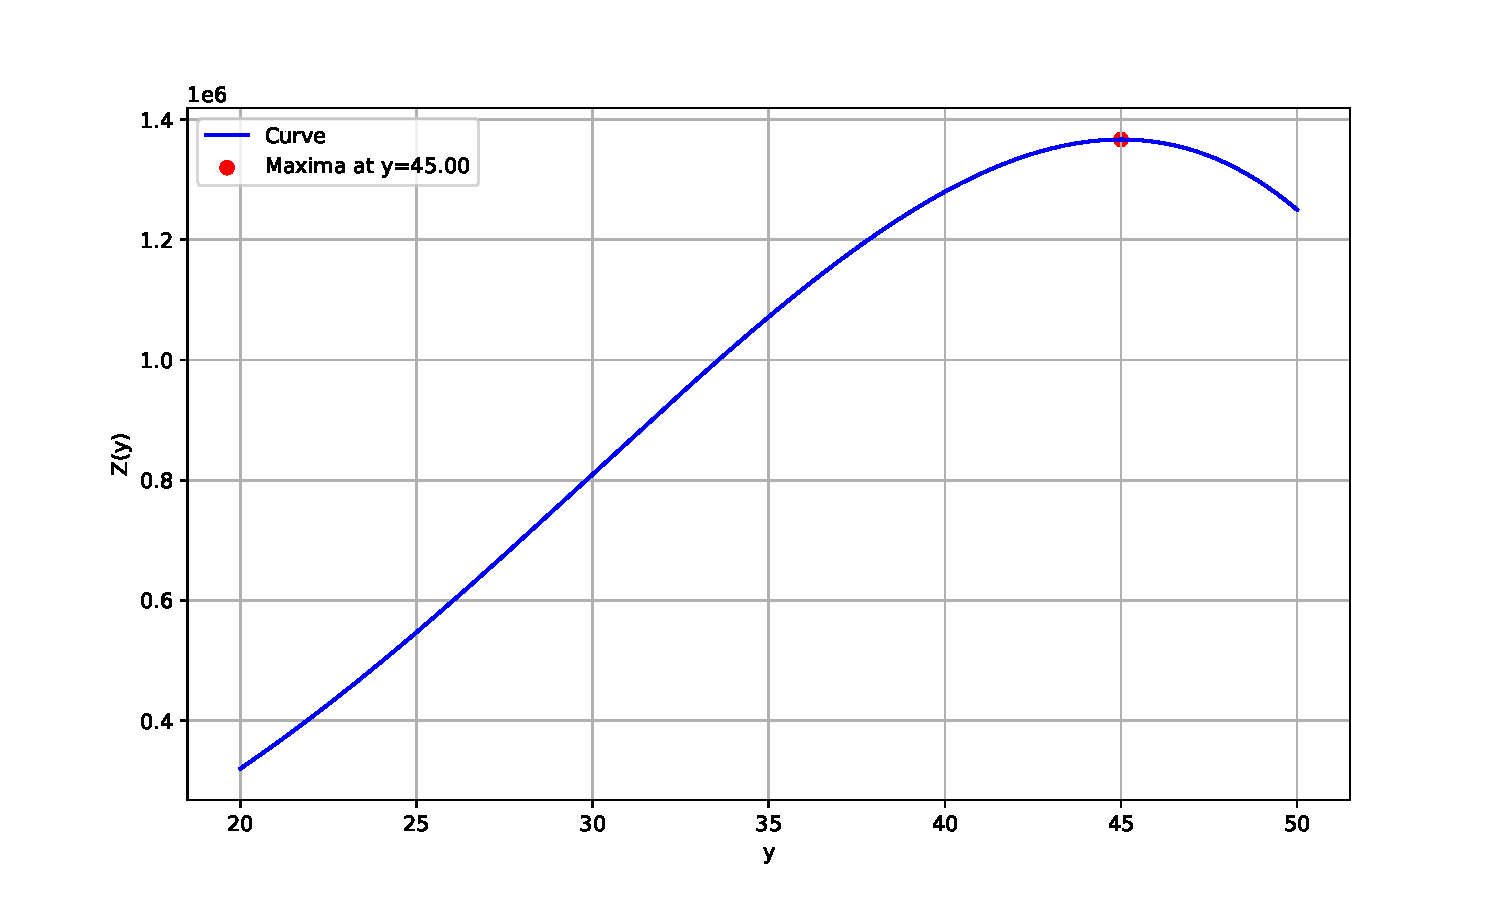
\includegraphics[width=\columnwidth]{figs/fig.pdf}
\end{figure}

\end{document}
